%!TEX root = ../../main.tex

\documentclass[../../main.tex]{subfiles}

\begin{document}
	\begin{tikzpicture}[scale=1.5]

		\coordinate (p1) at (0,0);
		\coordinate (p2) at (2,2);
		
		% Areas
		\draw [box] (-0.5,-0.5)--(1.4,-0.5)--(1.4,1.5)--(6.6,1.5)--(6.6,5.5)--(1.8,5.5)--(-0.5,5.5)--cycle;
		\fill [my_blue_2,opacity=0.4] (1.4,1.5) rectangle (6.6,5.5);

		% Init Position
		\fill [covered_area] (p1) circle [radius=0.5];
		\node at (p1) [right] {$q^0$};

		%Roomba$
		\node [inner sep=0pt,rotate around={-90:(p2)}] at (p2) {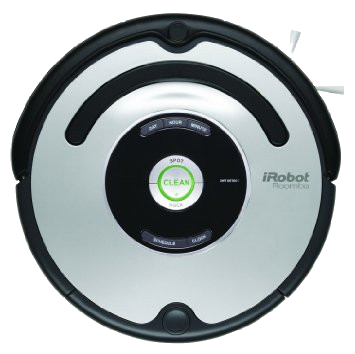
\includegraphics[width=.1\textwidth]{img/chapter_5/roomba.png}};

		% Init and return
		\draw [my_orange,opacity=0.5,line width=0.1cm] (p1)--(1.4,1.6)--(p2);
		\draw [my_orange,opacity=0.5,line width=0.1cm] (2,5)--(p1);
		\draw [dashed,->] (p1)--(1.4,1.6) -- (p2);
		\draw [dashed,->] (2,5)--(p1);

		\foreach \y in {2,3,...,5} {
			\draw [my_red, opacity=0.5,line width=0.1cm](2,\y)--(6,\y);
			%\draw [dashed] (2,\y)--(6,\y);
			\ifthenelse{\y=2 \OR \y=4}{\draw [dashed,->] (2,\y)--(6,\y);}{\draw [dashed,<-] (2,\y)--(6,\y);}
		}

		\draw [yellow,opacity=0.5,line width=0.1cm] (6,2) arc (-90:90:0.5);
		\draw [yellow,opacity=0.5,line width=0.1cm] (2,3) arc (270:90:0.5);
		\draw [yellow,opacity=0.5,line width=0.1cm] (6,4) arc (-90:90:0.5);
		\draw [dashed,->] (6,2) arc (-90:90:0.5);
		\draw [dashed,->] (2,3) arc (270:90:0.5);
		\draw [dashed,->] (6,4) arc (-90:90:0.5);


	\end{tikzpicture}
\end{document}